\documentclass[a4paper,11pt]{article}
% Various packages
\usepackage{siunitx}
\usepackage[utf8]{inputenc} % æøå
\usepackage[T1]{fontenc} % mere æøå
\usepackage[danish]{babel} % orddeling
\usepackage{verbatim} % så man kan skrive ren tekst
\usepackage{graphicx}
\graphicspath{{assets/}}
\usepackage{a4wide}
\usepackage{url}
\usepackage[left=2cm,top=2cm,bottom=1.5cm,right=2cm]{geometry}
\usepackage{amsmath}
\usepackage{amssymb}
\usepackage{amsthm}
\usepackage{wrapfig}
\usepackage{fixme}
\usepackage{color}
\usepackage{pstricks}
\usepackage{pdfpages} % include pdf
\usepackage{float} % Use [H] in figures
\usepackage{subcaption} % For subfigures
\usepackage{color} % May be necessary if you want to color links
\usepackage{hyperref} % Make references clickable
\usepackage[nameinlink,capitalize]{cleveref} % Make eq:refs be in style (1)
\usepackage[linesnumbered, commentsnumbered, lined, ruled, vlined,
%noend  % Have no ⌊-like symbol to indicate end of scope in pseudocode
]{algorithm2e} % Doc: https://goo.gl/6bC1qZ

% Ændr på navnene der vises når man bruger \autoref{label}
\def\sectionautorefname{Sektion}
\renewcommand{\equationautorefname}{Ligning}
\def\figureautorefname{Figur}
\AtBeginDocument{\renewcommand{\ref}[1]{\autoref{#1}}}

% Sæt \ref{} til at kalde \autoref{}
\AtBeginDocument{\renewcommand{\ref}[1]{\autoref{#1}}}

% Ændr ''*'' i math-felter til \cdot
\DeclareMathSymbol{*}{\mathbin}{symbols}{"01}

% Sæt farver for interne referencer og links
\definecolor{darkblue}{RGB}{25,25,112}
\hypersetup{
	colorlinks=true,    %set true if you want colored links
	linktoc=all,        %set to all if you want both sections and subsections linked
	linkcolor=darkblue, %choose some color if you want links to stand out
	filecolor=blue,     %
	citecolor=black,    %
	urlcolor=cyan,      %
}

% Set indentation to 0:
\setlength\parindent{0pt}

% Keywords relateret til algorithm2e pakken
\newcommand{\True}{\textbf{true}}\newcommand{\False}{\textbf{false}}
\SetStartEndCondition{ }{}{}%
\SetKwProg{Fn}{def}{\string:}{}
\SetKw{KwTo}{to}
\SetKwFor{For}{for}{}{}% 
\SetKwFor{ForEach}{foreach}{}{}% 
\SetKwIF{If}{ElseIf}{Else}{if}{}{elif}{else}{end}% 
\SetKwFor{While}{while}{}{end}\SetKwProg{Fn}{}{}{}
\SetKwInOut{Input}{input}\SetKwInOut{Output}{output}
\setlength{\algomargin}{3em}\DontPrintSemicolon

\newcommand{\longspace}{{\ \ \ \ \ \ \ \ \ \ \ \ \ \ }}
\renewcommand{\P}{{\mathbb P}}
\newcommand{\parfrac}[1]{\frac{\partial}{\partial #1}}
\renewcommand{\num}{{\textrm{num} }}
\newcommand{\size}{{\textrm{size} }}
\newcommand{\ift}{{\textrm{if } }}

% Dynamiske (), <>, ceil, floor
\newcommand{\p}[1]{\left( #1 \right)}
\newcommand{\pbig}[1]{\big( #1 \big)}
\newcommand{\pBig}[1]{\Big( #1 \Big)}
\newcommand{\pbigg}[1]{\bigg( #1 \bigg)}
\newcommand{\larr}[1]{\left< #1 \right>}
\newcommand{\ceil}[1]{\left\lceil #1 \right\rceil}
\newcommand{\floor}[1]{\left\lfloor #1 \right\rfloor}


% Squiggly arrows
\DeclareFontFamily{U} {MnSymbolC}{}

\DeclareFontShape{U}{MnSymbolC}{m}{n}{
	<-6> MnSymbolC5
	<6-7> MnSymbolC6
	<7-8> MnSymbolC7
	<8-9> MnSymbolC8
	<9-10> MnSymbolC9
	<10-12> MnSymbolC10
	<12-> MnSymbolC12}{}
\DeclareFontShape{U}{MnSymbolC}{b}{n}{
	<-6> MnSymbolC-Bold5
	<6-7> MnSymbolC-Bold6
	<7-8> MnSymbolC-Bold7
	<8-9> MnSymbolC-Bold8
	<9-10> MnSymbolC-Bold9
	<10-12> MnSymbolC-Bold10
	<12-> MnSymbolC-Bold12}{}

\DeclareSymbolFont{MnSyC} {U} {MnSymbolC}{m}{n}

\DeclareMathSymbol{\MNrhd}{\mathbin}{MnSyC}{76}
\DeclareMathSymbol{\MNlhd}{\mathbin}{MnSyC}{78}
% =============================================
\DeclareFontFamily{U} {MnSymbolD}{}

\DeclareFontShape{U}{MnSymbolD}{m}{n}{
	<-6> MnSymbolD5
	<6-7> MnSymbolD6
	<7-8> MnSymbolD7
	<8-9> MnSymbolD8
	<9-10> MnSymbolD9
	<10-12> MnSymbolD10
	<12-> MnSymbolD12}{}
\DeclareFontShape{U}{MnSymbolD}{b}{n}{
	<-6> MnSymbolD-Bold5
	<6-7> MnSymbolD-Bold6
	<7-8> MnSymbolD-Bold7
	<8-9> MnSymbolD-Bold8
	<9-10> MnSymbolD-Bold9
	<10-12> MnSymbolD-Bold10
	<12-> MnSymbolD-Bold12}{}

\DeclareSymbolFont{MnSyD} {U} {MnSymbolD}{m}{n}
\DeclareMathSymbol{\MNsim}{\mathbin}{MnSyD}{2}

% =============================================

\usepackage{amssymb,amsmath,stackengine}
\stackMath
\newcommand\rsquigarrow[1]{%
	\mathbin{\stackon[2pt]{\rightsquigarrow}{\scriptscriptstyle #1 }}
}

\author{Søren Mulvad, rbn601}

\title{Eksamensdisposition - Balancerede binære søgetræer}
\begin{document}
\maketitle

% Desuden skal hver studerende i gruppen udarbejde en individuel disposition for emnet "Binære søgetræer", som er et af emnerne til eksamen. En disposition skal bestå af de vigtigste punkter, du vil komme ind på til eksamen.
% Tænk på dispositionen som noget, du kan have med dig til eksamen, og som kan hjælpe dig med at huske, hvad du overordnet vil gennemgå til emnet "Binære søgetræer".
% Dispositionen skal ikke indeholde detaljerede beviser og lignende, men de mere overordnede delemner. Sørg for at gøre den kortfattet - f.eks. 5-10 punkter med stikord/-sætninger.

\begin{itemize}

\item \textbf{Motivation}


\item \textbf{Struktur for binære søgetræer}


\item \textbf{Struktur for rød-sorte træer}

\item \textbf{Bevis for at højden er $O(\lg n)$}


\item \textbf{Opretholdelse af egenskaber}



\end{itemize}

%%%%%%%%%%%%%%%%%%%%%%%%%%%%%%%%%%%%%%%%%%%%%%%%%%%%%%%%%%%
%%%%%%%%%%%%%%%%%%%%%%%%%%%%%%%%%%%%%%%%%%%%%%%%%%%%%%%%%%%
%%%%%%%%%%%%%%%%%%%%%%%%%%%%%%%%%%%%%%%%%%%%%%%%%%%%%%%%%%%
\newpage
%%%%%%%%%%%%%%%%%%%%%%%%%%%%%%%%%%%%%%%%%%%%%%%%%%%%%%%%%%%
%%%%%%%%%%%%%%%%%%%%%%%%%%%%%%%%%%%%%%%%%%%%%%%%%%%%%%%%%%%
%%%%%%%%%%%%%%%%%%%%%%%%%%%%%%%%%%%%%%%%%%%%%%%%%%%%%%%%%%%
\section{Balancerede binære søgetræer}



\begin{itemize}
\item \textbf{Motivation}
\begin{itemize}
	\item En effektiv datastruktur, som tilbyder worst-case garantier for ting som \texttt{Insertion}, \texttt{Deletion} og \texttt{Search}.
	\item Bliver f.eks. brugt i plane-sweep algoritmen (der ser om linjesegmenter skærer hinanden), samt i Linuxkernen og til at understøtte forskellige operationer i flere programmeringssprog.
\end{itemize}
	
	
\item \textbf{Struktur for binære søgetræer}
\begin{itemize}
	\item Attributer for hver knude: $key$ samt $left$, $right$ og $p$.
	\item Opsat så vi altid har $\leq$ elementer i venstre deltræ og $>$ elementer på højre deltræ.
	\item Mange operationer, inklusiv \texttt{Insert}, \texttt{Search}, \texttt{Delete} samt \texttt{Max} og \texttt{Min} kan nu udføres i $O(h)$ tid. Ved tilfældige indsættelser kan man vise at højden vil blive $O(\lg n)$, men vi er ikke altid garanteret at indsættelserne er tilfældige.
\end{itemize}

\item \textbf{Struktur for rød-sorte træer}
\begin{itemize}
	\item Ligesom binære søgetræer med den ene ekstra attribut $color$, som kan være rød eller sort. Løser problemet med at garantere en højde $h = O(\lg n)$.
	\item Opfylder 5 rød-sorte egenskaber:
	\begin{enumerate}
		\item Hver knude er enten rød eller sort
		\item Roden er sort
		\item Alle blade er $T.nil$, som er sort
		\item Hvis en knude er rød, så er begge dens børn sorte
		\item For hver eneste knude gælder, at alle simple veje fra knuden til dens efterkommere har det samme antal sorte knuder. Denne kalder vi $bh(x)$.
	\end{enumerate}
	\item Tegn figuren. Knudernes black-height $bh(x)$ er skrevet til venstre for dem:
	\begin{figure}[H]
		\begin{center}
			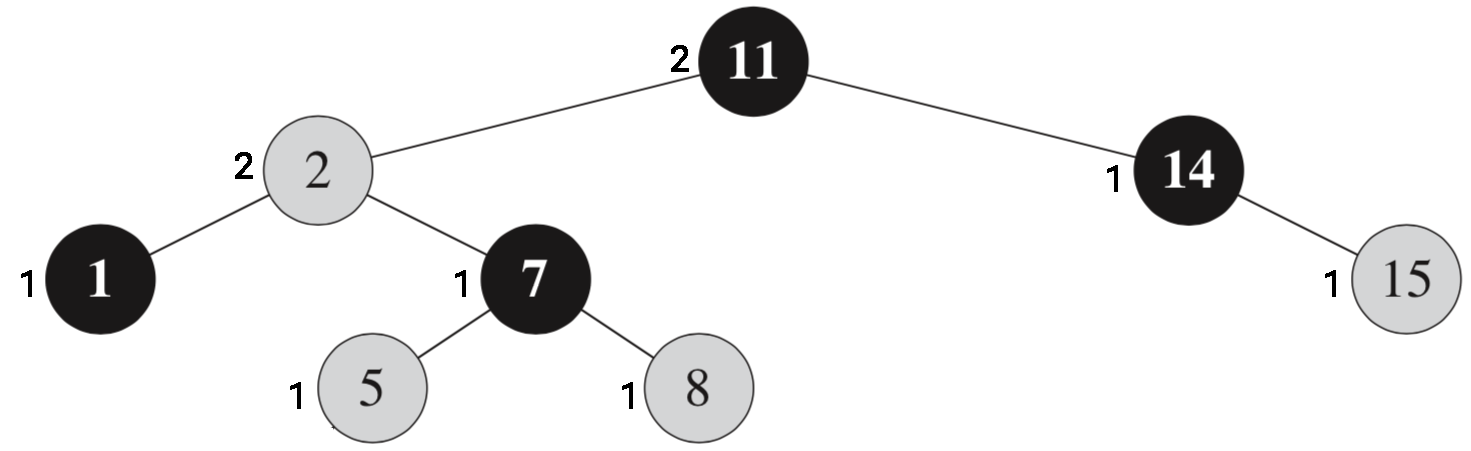
\includegraphics[width=0.65\textwidth]{rb.png}
		\end{center}
		%\caption{rb}
		\label{fig:rb}
	\end{figure}
\end{itemize}


\item \textbf{Bevis for at højden $h = O(\lg n)$ (s. 309)}
\begin{itemize}
	\item Jeg vil bevise, at et rødt-sort træ $x$ med $n$ interne knuder har en højde
	$$
	h = O(\lg n)
	$$
	\item Starter med Lemma. Lad $s(x)$ betegne antallet af interne knuder i et deltræ for knuden $x$. Vi starter så med ved stærk induktion at vise, at dette deltræ har mindst $2^{bh(x)} - 1$ interne knuder.
	\begin{equation} \label{eq:lemma}
	s(x) \geq 2^{bh(x)} - 1
	\end{equation}
	\item Base case ($x$ har en højde $h = 0$):
	\begin{itemize}
		\item $s(x) = 0$, da $x$ med den højde så må være et eksternt blad.
		\item $bh(x) = 0$ og derfor $2^{bh(x)} - 1 = 0$.
		\item Vi ser at \cref{eq:lemma} er overholdt.
	\end{itemize}
	\item Induktionsstep:
	\begin{itemize}
		\item Lad os nu sige knude $x$ har højde $h = k$. Så vil dens to børn $x.left$ og $x.right$ have en højde der højest er $k-1$. Pga. vores induktionsantagelse ved vi, at \cref{eq:lemma} gælder for dem. Vi får nu:
		\begin{align}
		s(x) &= s(x.left) + s(x.right) + 1\\
		     &\geq 2^{bh(x.left)} - 1 + 2^{bh(x.right)} + 1 \label{eq:child-to-bh} \\
		     &\geq 2^{bh(x)-1} - 1 + 2^{bh(x)-1} - 1 + 1 \label{eq:bh-min-1} \\
		     &= 2^{bh(x)} - 1 \label{eq:bh-lemma-done}
		\end{align}
		I \cref{eq:child-to-bh} benytter vi vores induktionsantagelse.\\
		I \cref{eq:bh-min-1} benytter vi, at et barn har en sort-højde $bh(x)$ (rød) eller $bh(x) - 1$ (sort).\\
		I \cref{eq:bh-lemma-done} lader vi to 1-taller gå ud med hinanden og sætter de potenser sammen.
	\end{itemize}
	\item Hermed har vi bevist vores Lemma. Nu skal bevise vores påstand. Vi benytter nu egenskab nr. 4, nemlig at hver rød knude har to sorte børn. Dvs. antallet af røde knuder på en vej fra roden ikke kan være med end $h/2$. Derfor må antallet af sorte knuder på sådan en vej minimum være $h/2$. Derfor får vi, at $bh(r) \geq h/2$.
	\item Nu samler vi disse uligheder hvorved vi får:
	\begin{align*}
	n = s(r) \geq 2^{bh(r)}& - 1 \geq 2^{h/2} - 1\\
	&\Updownarrow \\
	n + 1 &\geq 2^{h/2}\\
	\lg(n+1) &\geq h/2\\
	2\lg(n+1) &\geq h\\
	h &= O(\lg n)
	\end{align*}
	\item Det er hermed bevist.
\end{itemize}

\textbf{Opretholdelse af egenskaber:}\\
Jeg har hermed bevist, at højden på et RB-søgetræ er $O(\lg n)$. For at det skal gøre sig gældende er det meget vigtigt at vi overholder de fem egenskaber. Det kan vi gøre ved:
\begin{enumerate}
	\item LR (\texttt{Left-Rotation})
	\item RR (\texttt{Righ-Rotation})
	\item Farve en knude sort eller rød
\end{enumerate}

Vi kan have to cases når vi indsætter eller sletter en knude, det er:
\begin{enumerate}
	\item Vi overskrider ingen egenskaber og kan bare fortsætte
	\item Vi overskrider egenskaber, og skal rette op på det.
\end{enumerate}

Hvis det er case 2, så kan vi løse problemet lokalt, og hvis problemet bliver ved med at probagere op ad træet, helt op til roden er rød, så maler vi den bare sort.

\end{itemize}
\end{document}
